\section{Approach: Neuro-Symbolic Call-Graph Construction}
\label{sec:approach}

NSCG splits call-graph construction into the part that symbolic reasoning does
well --- enumerating every place that can call, naming things exactly,
following bindings and class hierarchies --- and the part where static
analyses are forced to over- or under-approximate --- deciding which of several
possible values reaches a call site, how a library behaves, and how an
outside callee is named. Figure~\ref{fig:pipeline} shows the three stages. S1
and S2 are deterministic Python code (about 1,200 lines, standard library only)
written for this project; N is a single LLM request per chunk of call sites.

\begin{figure*}[t]
  \centering
  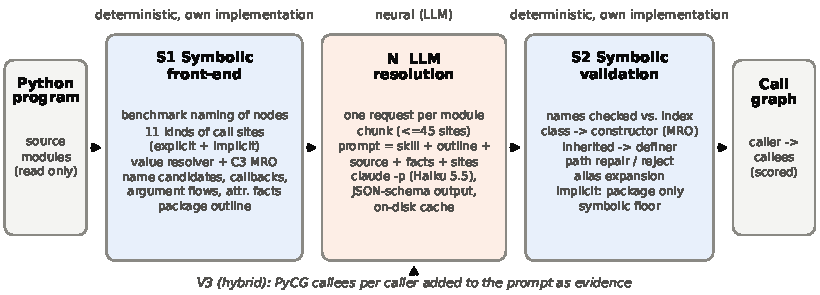
\includegraphics[width=0.92\textwidth]{figures/pipeline.pdf}
  \caption{Architecture of NSCG. S1 and S2 are symbolic and deterministic; N is
  the only neural stage. The hybrid variant V3 additionally shows PyCG's
  callees to the LLM.}
  \label{fig:pipeline}
\end{figure*}

\subsection{S1: symbolic front-end}
\label{sec:s1}

The front-end parses every module with Python's \texttt{ast} module (code is
never imported or run) and computes:

\textbf{Nodes with benchmark names.} Modules, functions, methods and lambdas
get the dotted names of the conventions; a lambda is numbered by the source
position of its \texttt{lambda} keyword among the lambdas of the scope that
evaluates it, and class bodies and comprehensions are transparent for the
caller attribution. On the four packages our node sets equal the ground-truth
node sets exactly (634 nodes); on the micro-benchmark they are equal in 613 of
622 cases (the others contain modules that never run).

\textbf{Call sites.} A walker attributes each site to the node whose execution
makes it (a decorator or default value to the enclosing scope, a class body to
the function or module that runs it). It finds 13 kinds of sites: explicit
calls, decorators, \texttt{raise C} without a call, and class creation
(\texttt{\_\_init\_subclass\_\_}, metaclass hooks, \texttt{\_\_set\_name\_\_}),
plus nine implicit kinds: \texttt{with}, iteration (\texttt{for},
comprehensions, \texttt{yield from}, unpacking), \texttt{**} mappings,
\texttt{await}, operators (binary, augmented, unary, comparisons and
\texttt{in}), subscripts (get/set/del), property accesses, truth tests and
f-string formatting. An implicit site is kept only if some package function has
a matching special-method name, because only package callees of implicit calls
are edges. The four packages yield 1,973 sites (the ground-truth ledgers have
1,846 sites of the kinds that need an entry).

\textbf{Symbolic pre-resolution.} A flow-insensitive, demand-driven resolver
maps an expression to abstract values: package functions, bound methods,
decorated definitions, classes, instances, modules, \texttt{super()} objects,
parameters, and outside paths/instances. Names are looked up through Python's
scoping rules (local, enclosing, \texttt{global}/\texttt{nonlocal}, module,
builtins), imports including relative and star imports, assignments (followed
recursively up to depth~6), the C3 MRO of package classes (an outside base
terminates the lookup and names the member through that base), instance
attributes through \emph{attribute facts} (\texttt{self.x = e} in any class of
the receiver's hierarchy), and return expressions of called functions. A call of
a class targets what instantiation runs (first \texttt{\_\_init\_\_} of the MRO,
inside or named through the nearest outside base, a package
\texttt{\_\_new\_\_}, a metaclass \texttt{\_\_call\_\_}). A resolution is
marked \emph{certain} when the callee is a static path with one binding (a
plain name bound once, or an attribute chain on a module).

\textbf{Candidates and facts.} The resolver is deliberately cheap, so it misses
values. To give the LLM a complete menu, every site also gets (i) the package
functions whose name equals the called name, the constructors of package
classes with that name, and the overriding methods of the receiver class's
package subclasses (receivers can be subclass instances); (ii) the package
functions and classes passed as arguments (callbacks); (iii) for a call of a
parameter, the package functions that resolved package calls pass for that
parameter (one level of argument flow); (iv) the attribute assignments that
matter for the chunk's attribute calls; and (v) a symbolic outline of the
whole package (imports, functions with parameters and decorators, classes with
bases, MRO, methods, properties and class attributes) used for naming callees
in other modules. \emph{V2.1 only:} at a call of a library method on a package
instance whose class derives from that library, (vi) the methods of the
package's subclasses of that library's classes, which the library may call back
(template methods, hooks).

\subsection{N: LLM resolution of call sites}

The sites of a module are split into chunks of at most 45, and each chunk
becomes one request. The prompt contains: a fixed ``skill'' that restates the
call-graph semantics in 40 lines (node names, which implicit calls and
callbacks are edges, the MRO rule for constructors, how outside callees are
named); instructions on how to treat the symbolic information (pre-resolutions
are usually right when certain, name candidates are naive and must be filtered
by types and hierarchy, implicit sites admit only package callees, never invent
a package name); the outline and the attribute facts; the numbered source of
the module (or, for modules above 700 lines, the window that holds the chunk's
callers plus the import header); and one line per site with its id, caller,
position, kind, text and symbolic information. The model answers a JSON object
\texttt{\{"sites": [\{"id", "callees"\}]\}}, enforced by a JSON schema.

We run the model through headless Claude Code (\texttt{claude -p}) with all
tools disabled, no settings, no project memory and an empty working directory,
so each request is a pure, stateless LLM call; Claude Code here is only the
transport and the structured-output enforcement. The default model is Claude
Haiku~5.5 (the cheapest current Claude model); we also report Claude
Sonnet~5.5. Every request and answer is stored in a content-addressed cache,
so all reported numbers can be replayed offline, and its token usage and cost
are recorded.

\subsection{S2: symbolic validation}

The model's names are checked against the definition index of S1. A name that
is a package node is kept; a package class is replaced by what instantiating it
runs; \texttt{pkg.C.m} for a method that \texttt{C} inherits is mapped through
the MRO to the defining class; a package-looking name that names nothing is
repaired if exactly one node shares its last two components (a wrong module
path) and is otherwise rejected as a hallucination; an outside name whose head
is a local import alias is expanded; at implicit sites outside names are
dropped; and, as a \emph{symbolic floor}, certain resolutions of S1 are always
kept. If the model omits a site, its symbolic resolution is used. Every
decision is counted (Table~\ref{tab:validation}).

\subsection{Variants and design iterations}
\label{sec:variants}

To find out which components matter, we built the design incrementally and
kept each version as a variant that runs on the same subjects:

\begin{itemize}[leftmargin=*]
\item \textbf{S1-only} (\texttt{nscg-sym}): the symbolic pre-resolutions alone,
no LLM --- the symbolic half of NSCG as an analysis of its own.
\item \textbf{V0, LLM-only}: the model receives the skill, the outline and the
source and writes the call graph \texttt{\{caller: [callees]\}} directly. This
is the obvious way to use an LLM and our neural reference point.
\item \textbf{V1, sites without hints}: S1 enumerates the sites, but the prompt
contains no per-site symbolic information and no facts; S2 validates.
\item \textbf{V2, NSCG}: the full design of Sections~\ref{sec:s1}--S2.
\item \textbf{V2.1}: the revision after the error analysis of V2
(Section~\ref{sec:rq3}): library-hook candidates (vi) and three fixes of the
validator's alias expansion that wrongly rewrote correct names
(\texttt{time.time}$\rightarrow$\texttt{time.time.time} after \texttt{from time
import time}, \texttt{invoke.Argument}$\rightarrow$\texttt{invoke.\_\_version\_\_.Argument}
after \texttt{from invoke import \_\_version\_\_ as invoke}, and
\texttt{builtins.all} instead of \texttt{<builtin>.all}).
\item \textbf{V3, hybrid}: V2/V2.1 plus, for each caller of the chunk, the
callees that PyCG-2026 reports, presented as evidence that can be wrong.
We also evaluate the offline set combinations PyCG\,$\cup$\,NSCG and
PyCG\,$\cap$\,NSCG.
\end{itemize}

\subsection{What is original, and relation to prior work}

All of S1, S2, the prompts, the skill text, the variants and the evaluation
scripts were written for this project. We reuse only infrastructure: the
benchmark, its ground truths, its runner and scorer (so that every tool is
scored identically), PyCG itself as the baseline and as the evidence source of
V3, and Claude Code as the LLM transport. The design is related to, but
differs from, prior neuro-symbolic work. Learned call-graph pruning
(CGPruner~\cite{utture2022cgpruner}, AutoPruner~\cite{le2022autopruner})
removes edges from a sound static graph with a classifier; NSCG instead lets
the LLM choose among symbolic candidates and add callees, and its symbolic
stages constrain the LLM rather than the other way round. LLM-based data-flow
analysis such as LLMDFA~\cite{wang2024llmdfa} and LLM-assisted static bug
detection such as LLift~\cite{li2024llift} and IRIS~\cite{li2025iris} use the
LLM for sources, sinks, summaries or path feasibility of a different analysis
task; NSCG uses it for value resolution at call sites and constrains it with a
generated candidate menu and a symbolic validator. Studies that ask LLMs for
Python call graphs on micro-benchmarks~\cite{venkatesh2024emergence} evaluate
our V0 setting; we compare it with our neuro-symbolic design on real packages.
